%% Use the hmcposter class with the thesis document-class option.
\documentclass[thesis]{hmcposter}
\usepackage{graphicx}
\usepackage{natbib}
\usepackage{booktabs}
\usepackage{subfig}
\usepackage{amsmath}
\usepackage{textcomp}
\usepackage{url}
\usepackage{enumitem}
\setlist{leftmargin=2cm, labelsep=0.7cm}

%% Author of the thesis.
\author{Stetson Bost}

%% The year of your thesis poster's creation.
\posteryear{2017}

%% Thesis Title.
\title{Adaptive Nested Algorithms\\for Balanced Scheduling}

%% Advisor name.
\advisor{Weiqing Gu}

%% Define the \BibTeX command, used in our example document.
\providecommand{\bibtex}{{\rmfamily B\kern-.05em%
    \textsc{i\kern-.025em b}\kern-.08em%
    T\kern-.1667em\lower.7ex\hbox{E}\kern-.125emX}}


\pagestyle{fancy}

\begin{document}

\begin{poster}

\section{Introduction}
Scheduling is very important for staying organized and managing stress for both individuals and all kinds of organizations.
For this project, we developed algorithms that create effective, adaptable, and balanced schedules.

\section{Algorithm for Personal Scheduling}
Our nested algorithm for creating personal schedules aims to mimic human behavior using machine learning to schedule tasks with deadlines while maintaining a balanced schedule.
We define a \emph{schedule} to be a collection of relatively short \emph{time slots}, with contiguous time slots forming \emph{blocks}.
We define a \emph{section} to be a group of blocks.
Our algorithm has three nested steps.
\begin{enumerate}
	\item
		Assign tasks to sections, prioritizing tasks according to their deadlines so that all tasks are completed on time, if possible.
	\item
		Assign tasks to blocks within sections, prioritizing a balance of intensity levels among blocks.
	\item
		Assign tasks to time slots within blocks in a way that can adapt to personal needs and preferences.
\end{enumerate}
Each step takes into account various aspects of the tasks, including deadlines, estimated duration, and intensity. Additionally, each block has a minimum permissible amount of time reserved for non-work activities. This can be used for structured activities, such as doing laundry or preparing a meal, or it may be unstructured personal time, depending on user preference.
By maintaining similar intensity levels among blocks, the algorithm favors a balanced schedule.

%TODO distribute important tasks to section Assign important tasks first
% try to balance within sections, talk about 
% Assign medium tasks to blocks by taking balance into consideration
% tasks to timeslots considering personal needs (ADAPTIVE)
\begin{figure}
  \centering
        \subfloat[][Start with a list of tasks that need to be completed. Each task has a deadline, estimated duration, and an intensity level, where a higher intensity level corresponds to a more difficult or stressful task.]{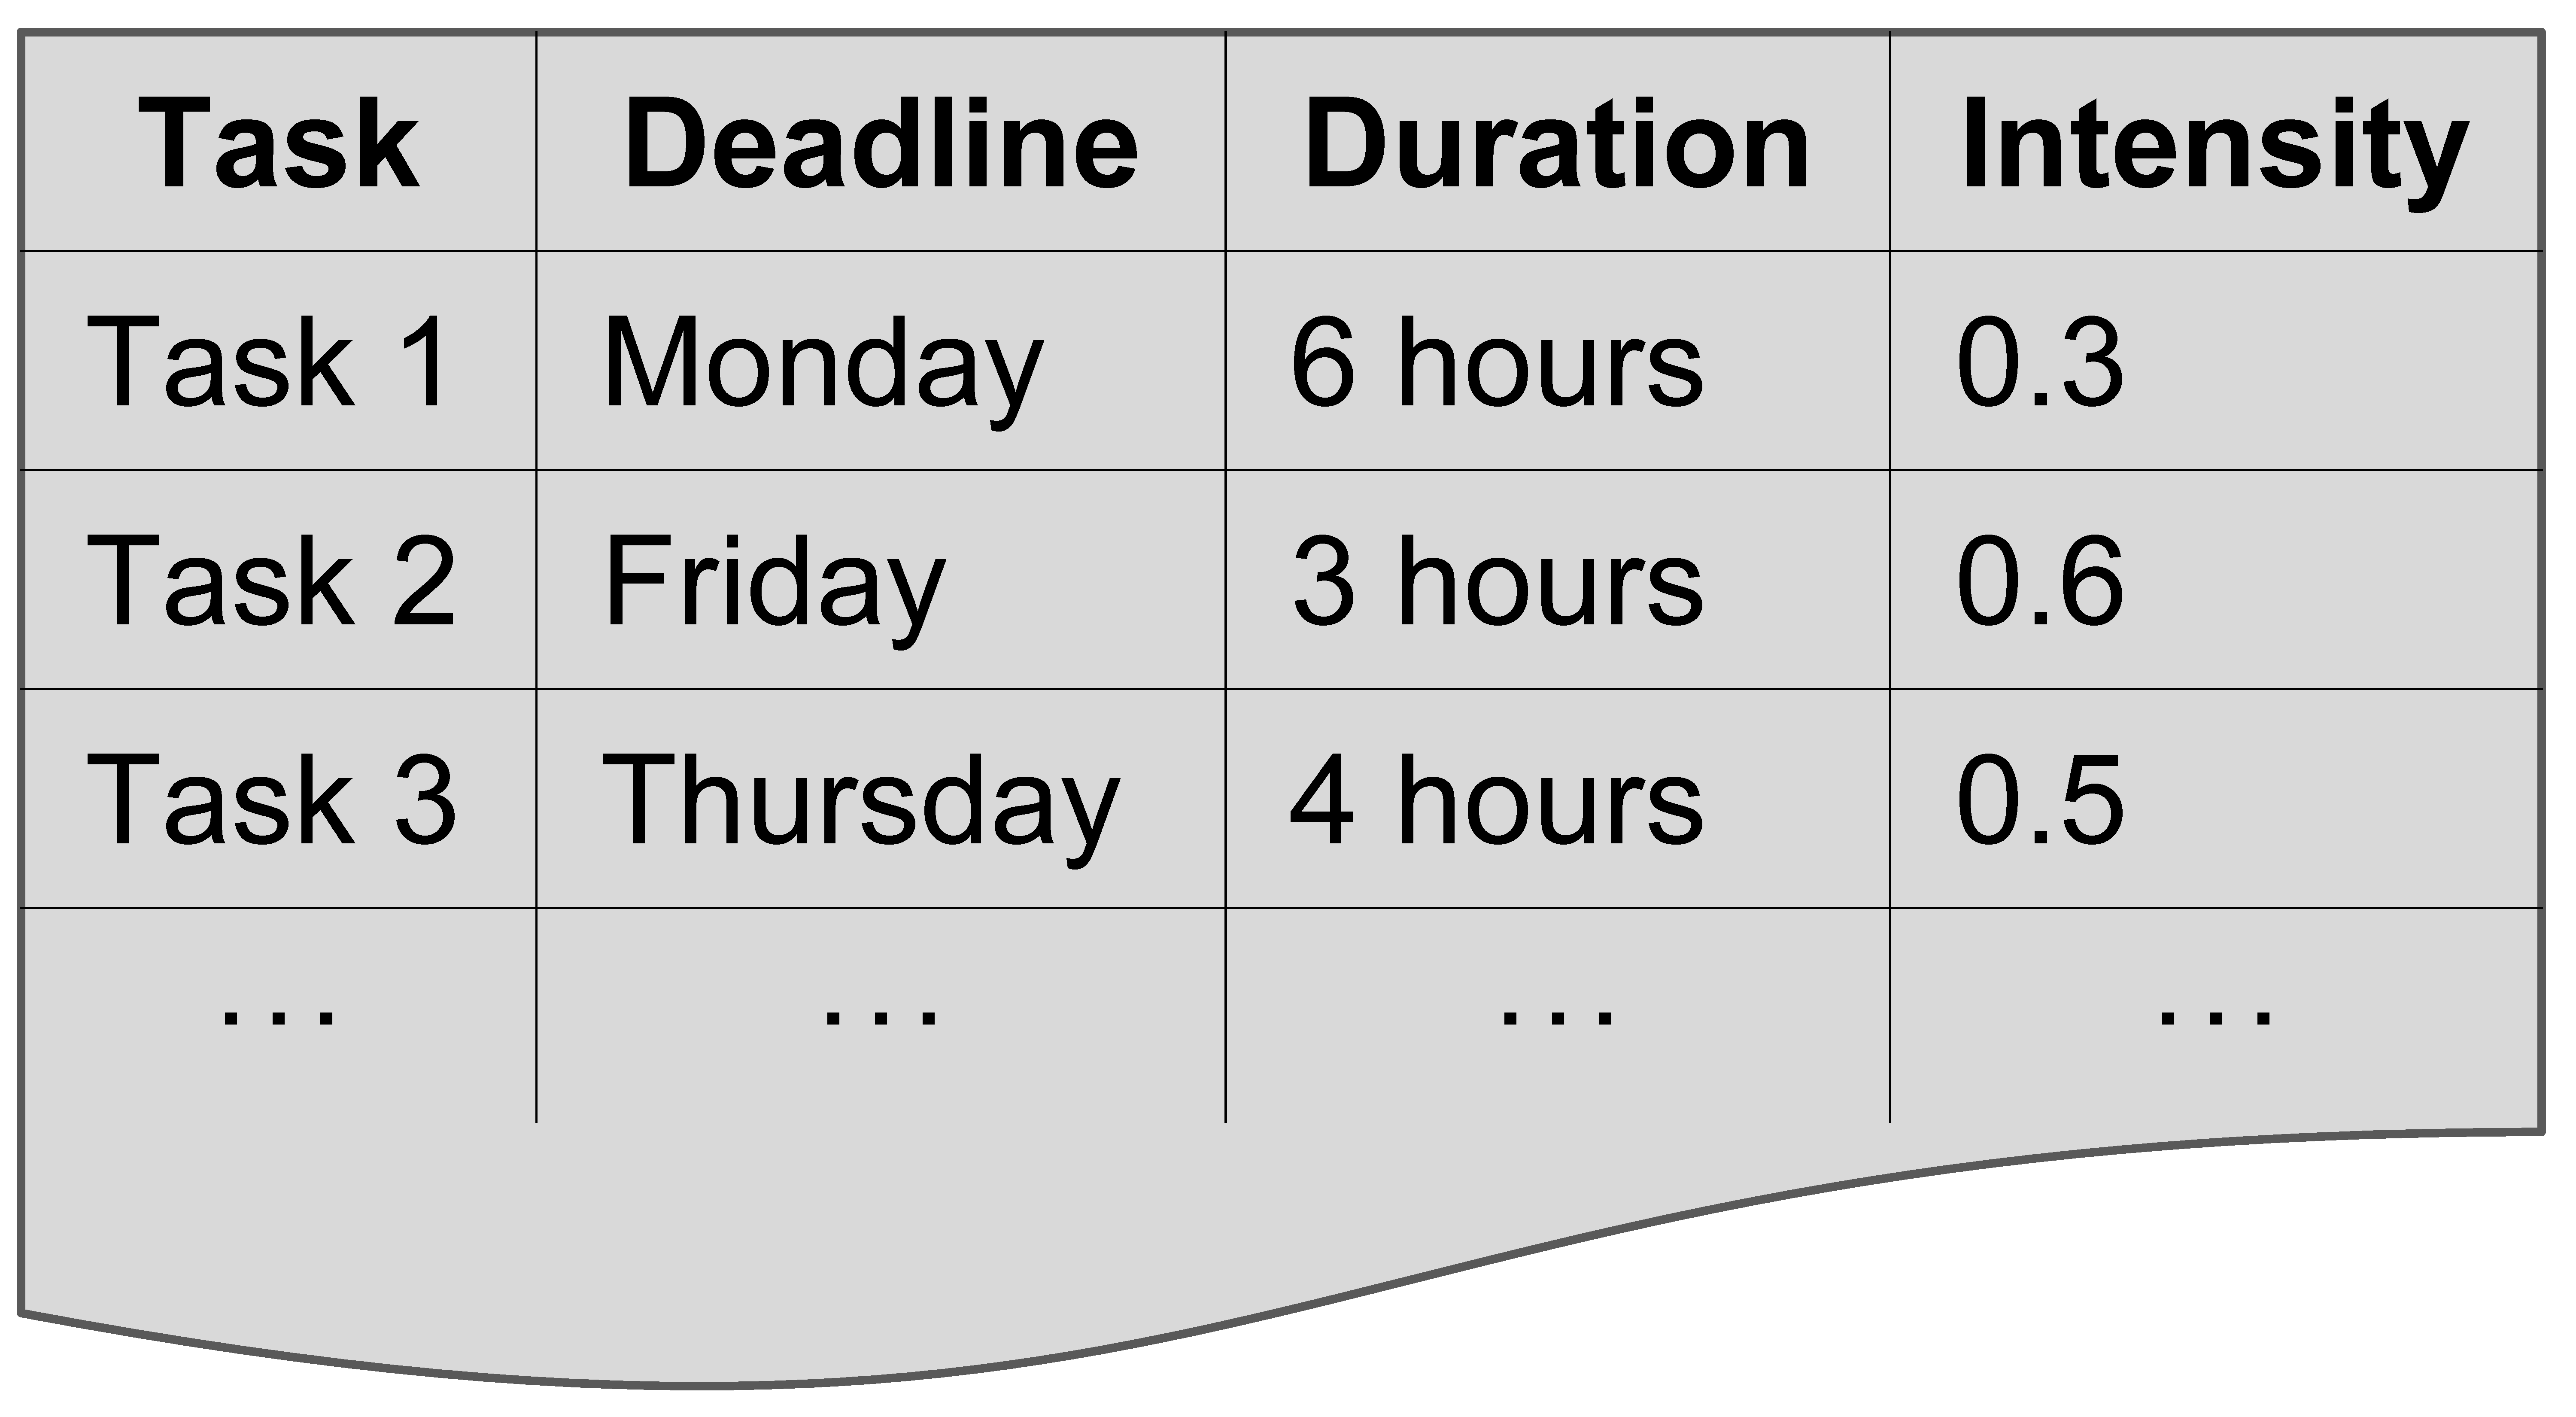
\includegraphics[scale=0.152]{TaskList.pdf}%
                \label{fig:small-mults-orig}%
        }\qquad\qquad
        \subfloat[][Step 1: Create a section made up of time blocks, and assign tasks to the section, prioritizing tasks with the soonest deadlines. Some amount of non-work time is associated with each block, and we treat non-work time as a task.]{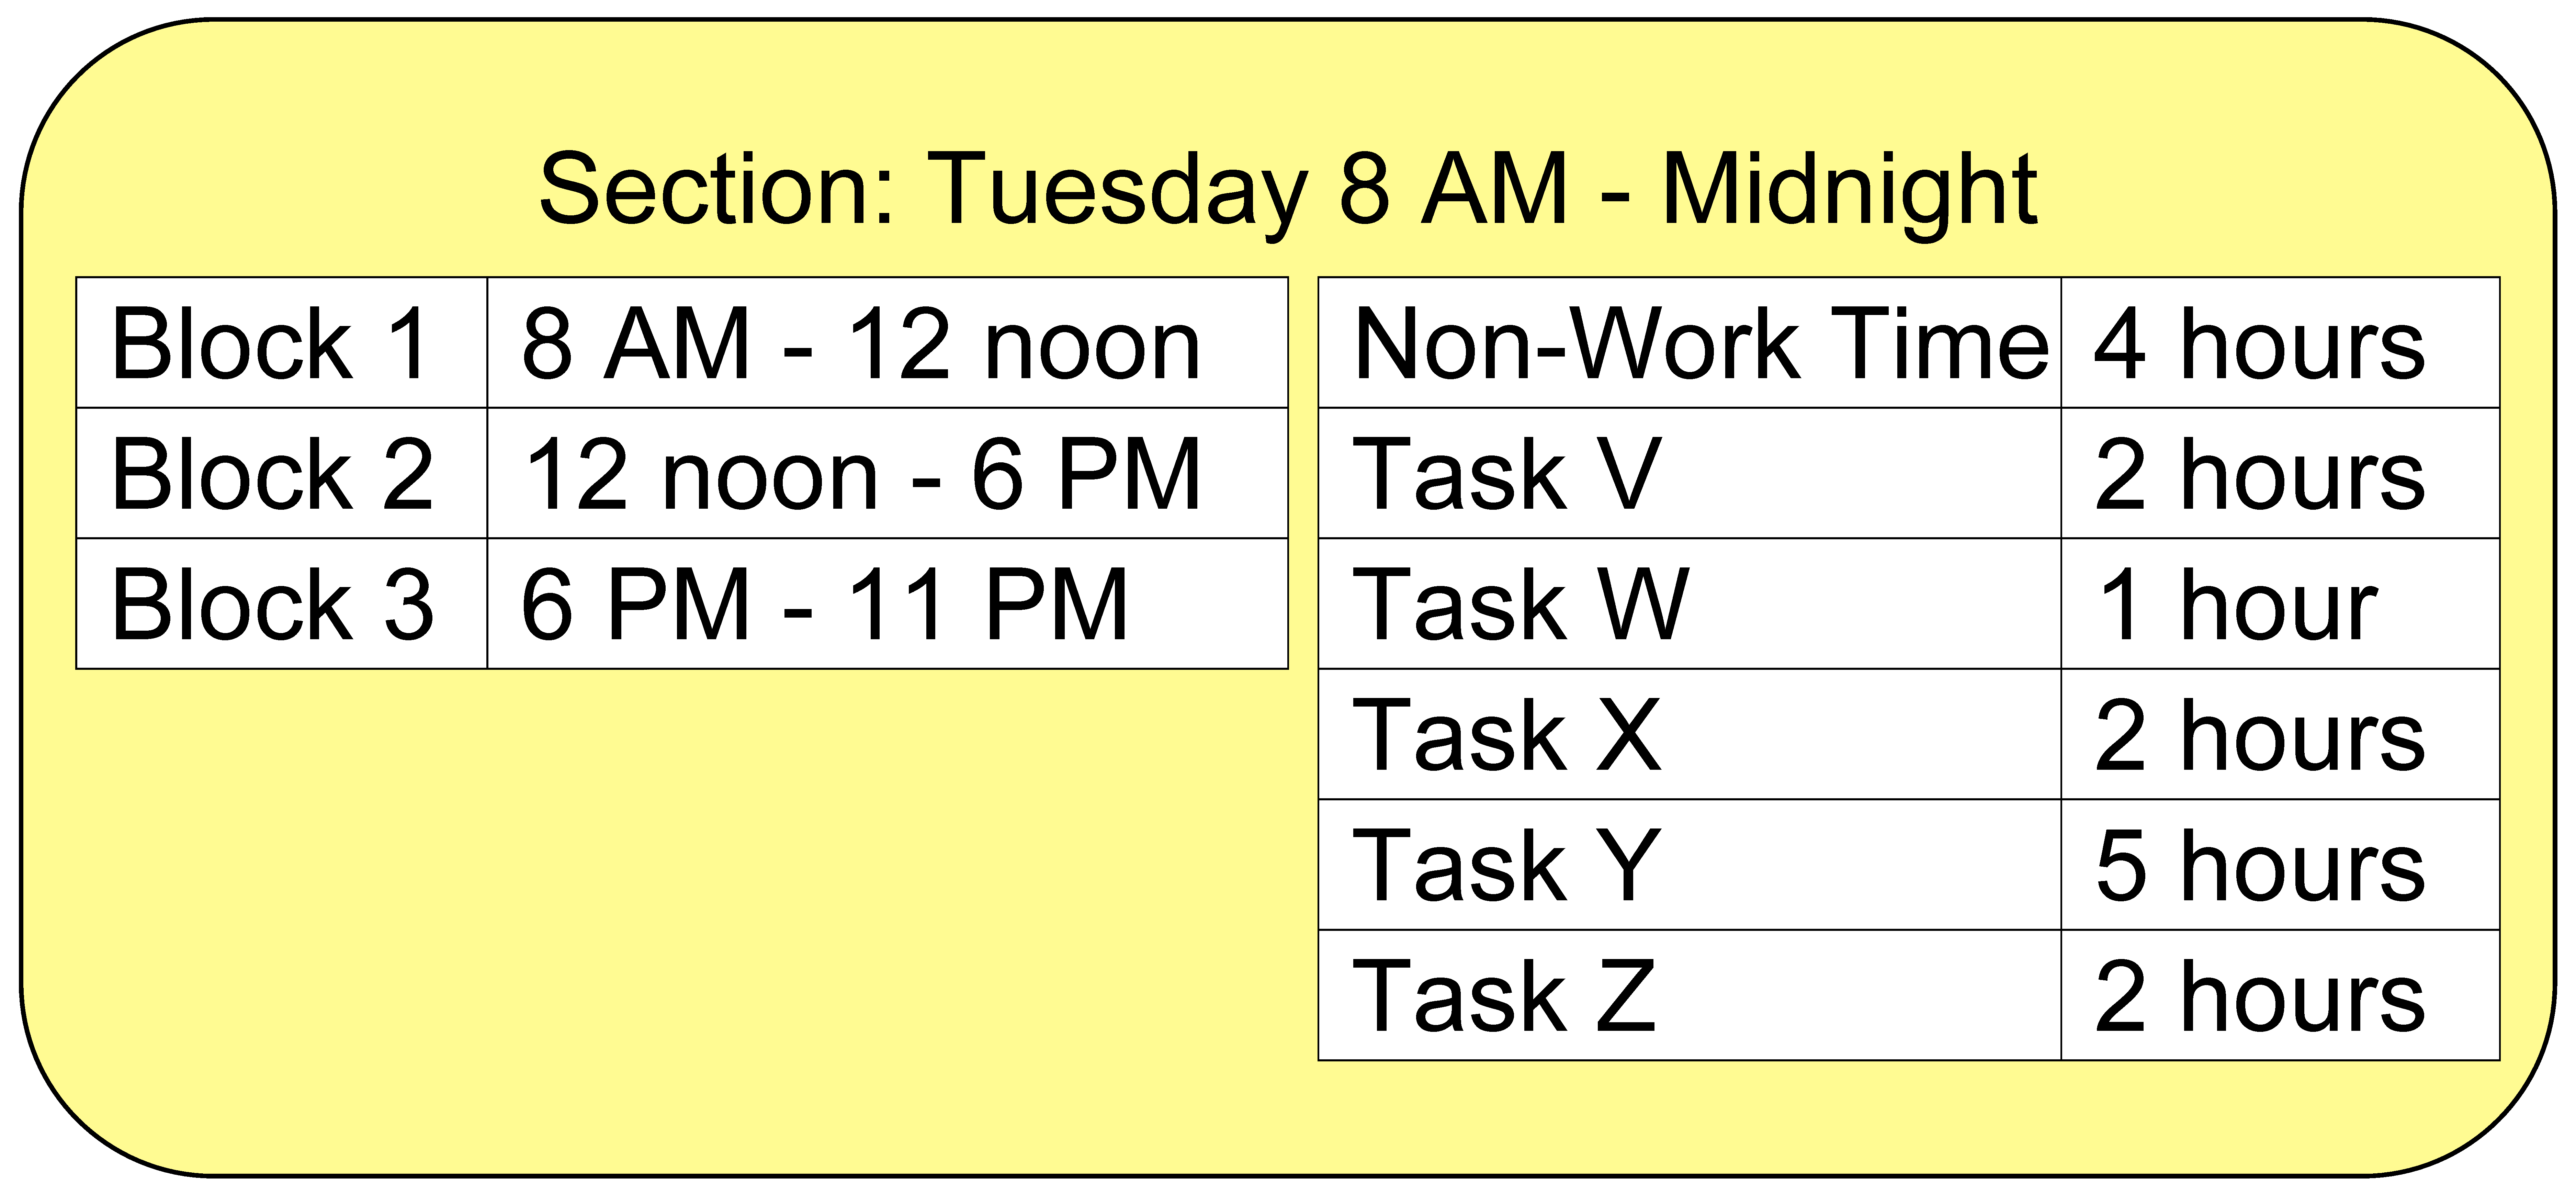
\includegraphics[scale=0.152]{Section.pdf}%
                \label{fig:small-mults-45}%
        }\\
        \subfloat[][Step 2: Assign tasks to each block in the section, prioritizing a balance of intensity levels from block to block.]{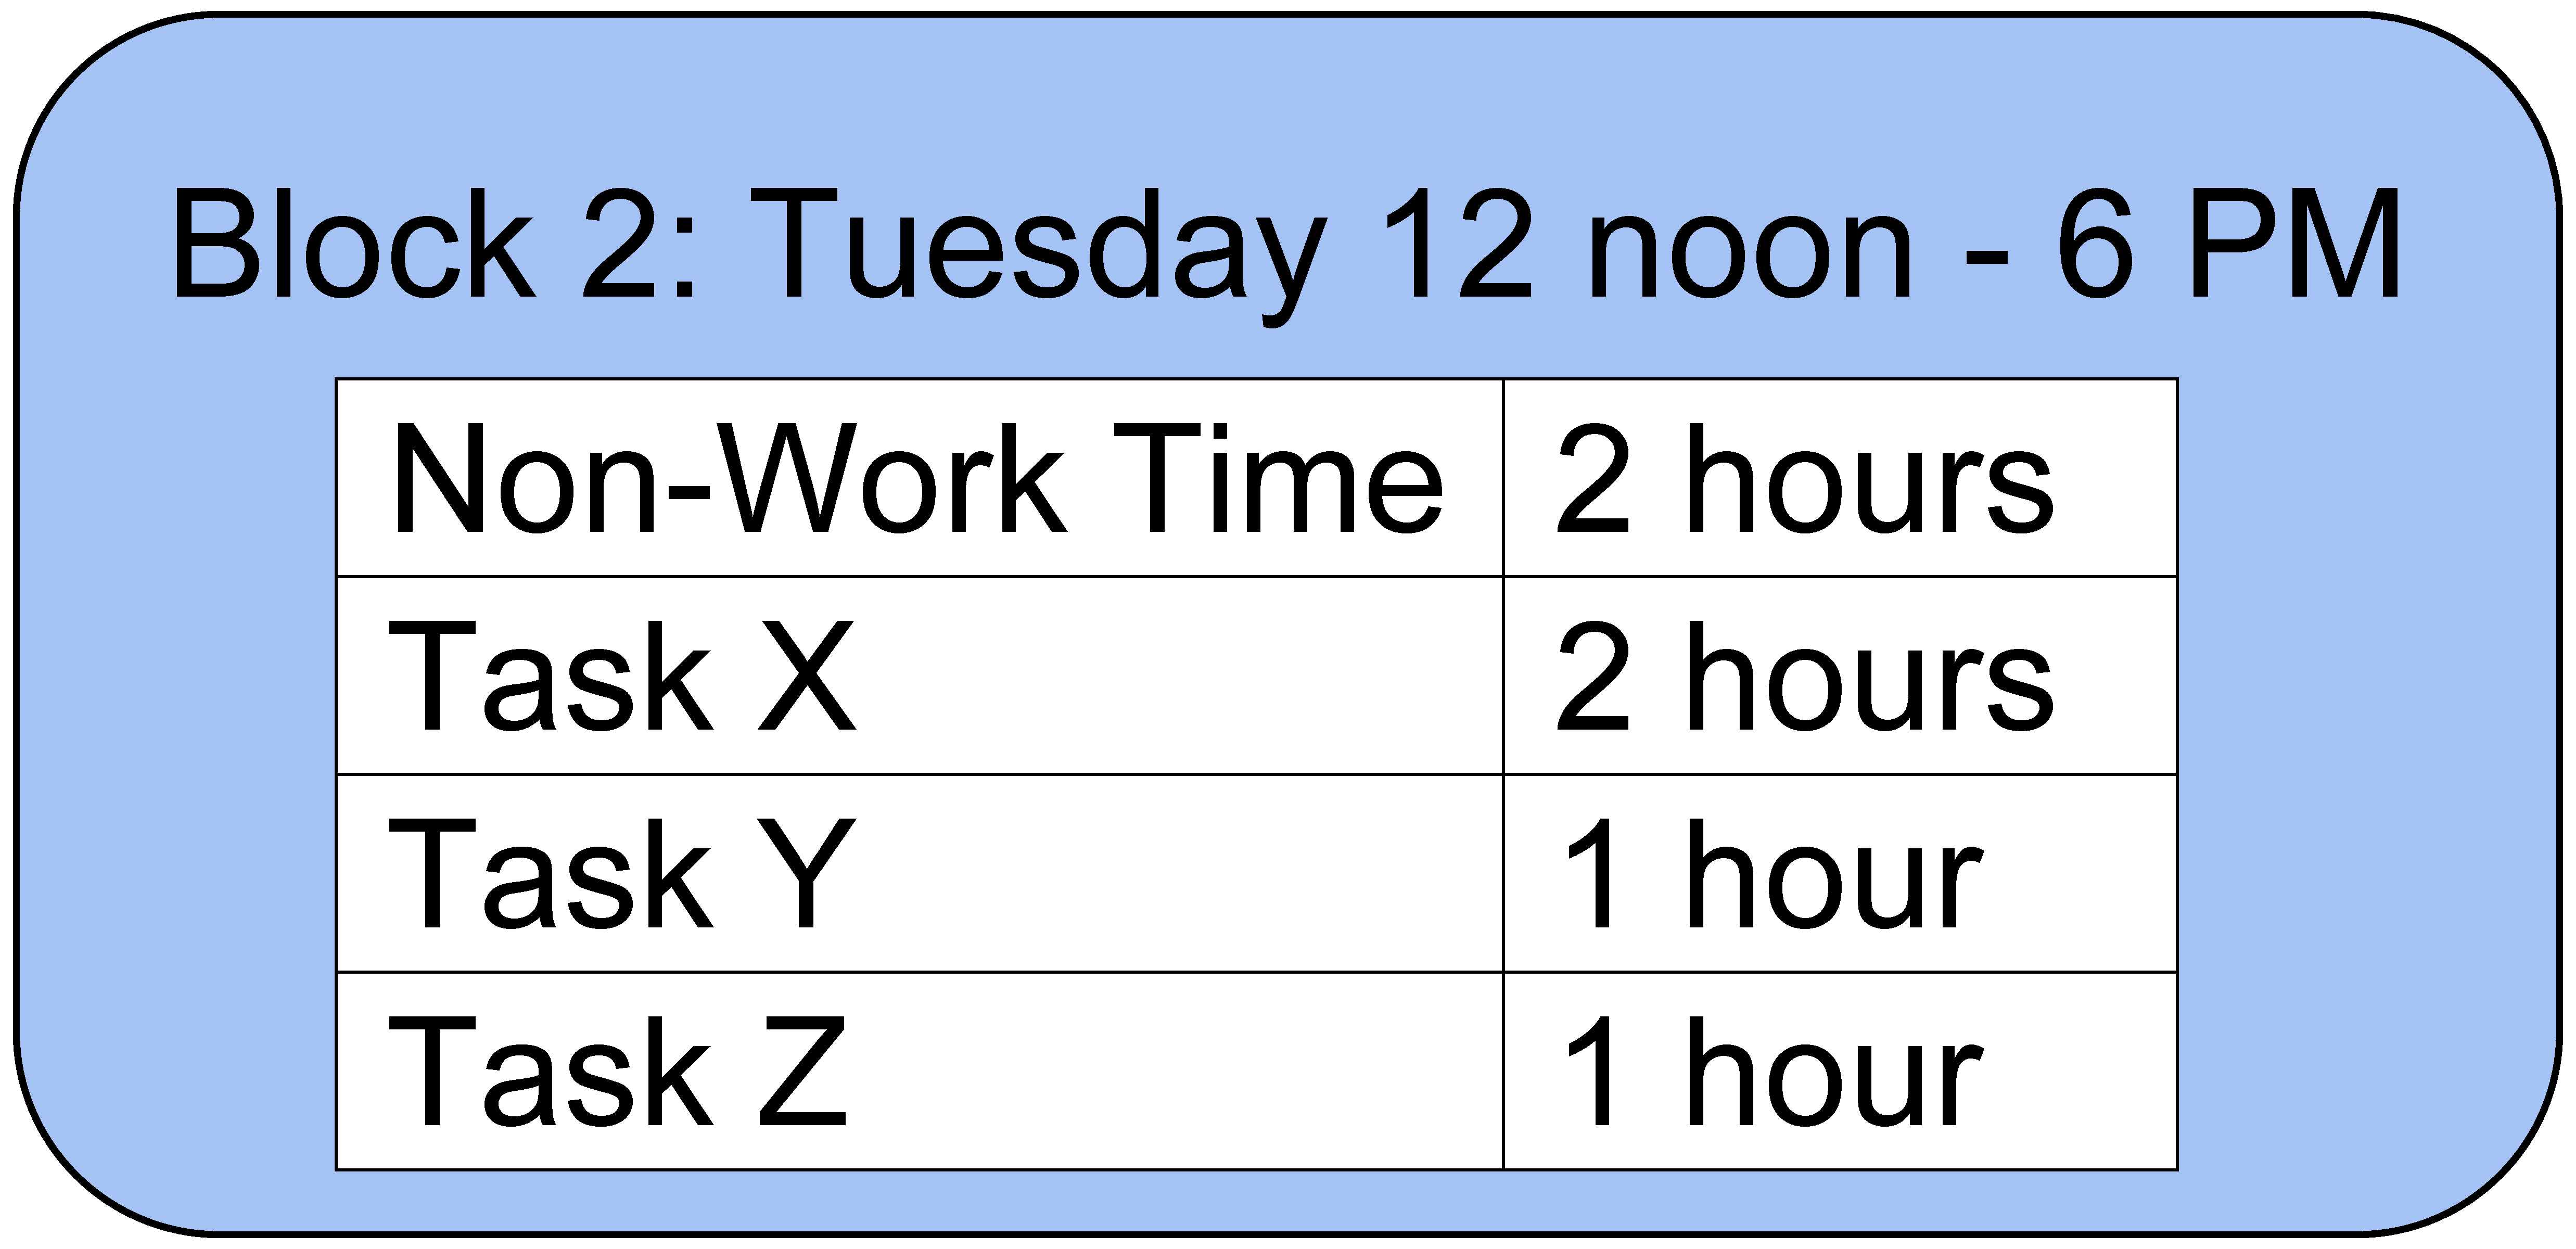
\includegraphics[scale=0.152]{Block.pdf}
        }\qquad\qquad
        \subfloat[][Step 3: Schedule tasks within the block. This step can be done in any way the user prefers. ]{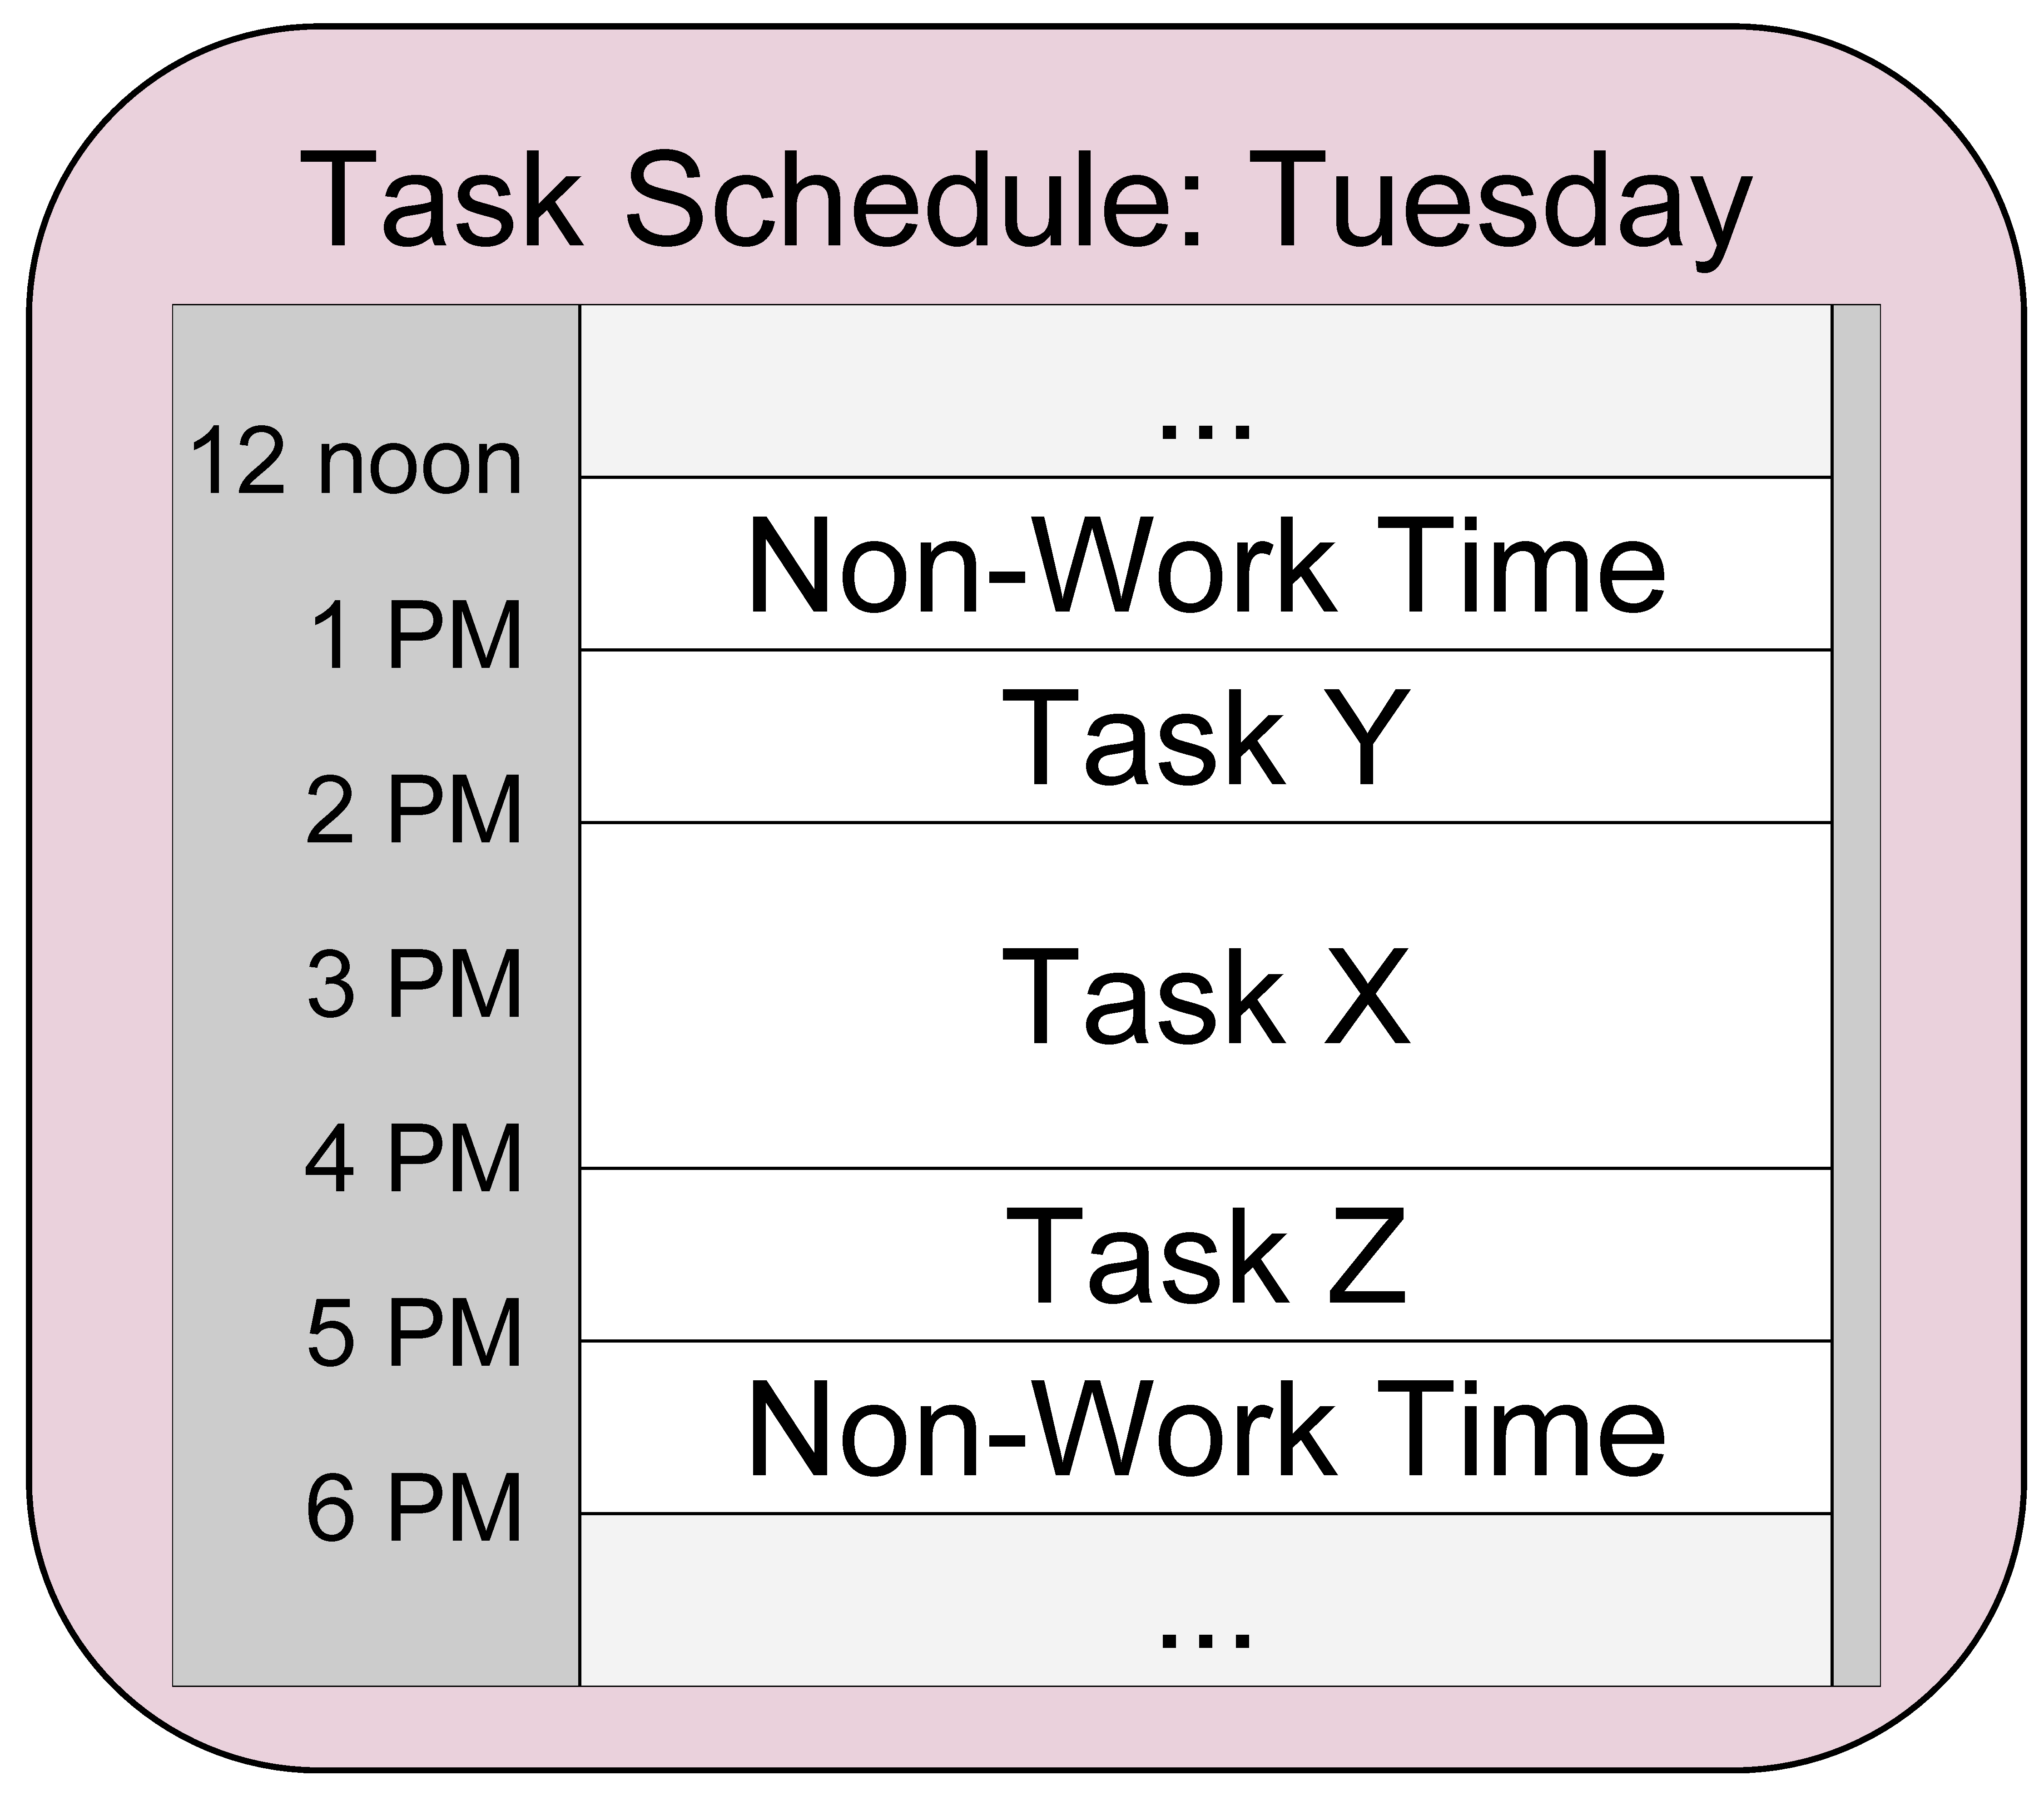
\includegraphics[scale=0.152]{Schedule.pdf}
        }
  \caption[]{Example of the personal scheduling algorithm, focusing on a section containing three blocks on Tuesday.}%
  \label{fig:small-multiples}
\end{figure}



\section{For Further Information}
For more information about this project, please contact \url{sbost@hmc.edu} or \url{gu@hmc.edu}.
%\columnbreak


\section{Algorithm for Event Scheduling}
We developed two algorithms for scheduling events within groups.
Members of a group often have to arrange events where a number people must attend.
An event may be either recurring (``regular'') or non-recurring (``special''), may have restrictions on available times, and may have a list of desired or required attendees.

\subsection{Probabilistic Approach}
We created an algorithm for event scheduling that uses historic data and a probabilistic version of the $k$-nearest neighbors algorithm to determine the likelihoods that all potential attendees will attend a specific event scheduled at potential times (Holmes and Adams, 2002).
By summing these likelihoods across all attendees, we are able to get the expected value for the number of people at the event.

\subsection{Nested Approach}
We also developed a nested algorithm that makes use of the nested personal scheduling algorithm detailed to the left with some slight modifications.
The basic structure of time slots, blocks, and sections is the same, but it may be less likely to have adjacent blocks or contiguous sections, depending on the group's scheduling practices.
We treat events as tasks with possible time windows, and use those to create sections.
In place of task intensity, we use a quantity that describes the priority of the event.
We also introduce some conditions for balance, such as restrictions on the frequency of regular and special events.


\section{Discussion and Future Work}
We are in the process of running the algorithms with a large data set.

In the future, these algorithms could be used with people and groups that are willing to try schedules that are produced.
Additionally, for an organization that uses a common calendar application, it might be possible to integrate the event scheduling algorithms with the calendar to automatically schedule events.


\section{References}
\bibliographystyle{hmcmath}
%\bibliography{sampleposter}
Holmes, C.~C.~and Adams, N.~M. (2002) A probabilistic nearest neighbour method for statistical pattern recognition. \emph{J.~R.~Statist.~Soc}. \textbf{64}, Part 2, pp.~295--306.
 \url{http://hedibert.org/wp-content/uploads/2016/02/holmes-adams-2002.pdf}.


\section{Acknowledgments}
I would like to thank my advisor, Professor Weiqing Gu, for her guidance throughout this research.
I am also very grateful for the kindness and generosity of the Rose Hills Foundation through their Science and Engineering Summer Undergraduate Research Fellowship, which has made this project possible.


\end{poster}

\end{document}

 
